\section{Space Imaging Simulator for Proximity Operations} \label{sec:sispo}
\gls{sispo} is a software package that integrates trajectory simulation with physics-based rendering, image compression and \gls{3d} reconstruction. These functionalities are split into three sub-packages. The first sub-package uses Keplerian orbit data for a \gls{sssb} and a definition of the encounter geometry for the spacecraft to propagate both on realistic trajectories and render an image series of the encounter. The second sub-package provides various algorithms for image compression and decompression. The third sub-package uses images to reconstruct a textured \gls{3d} model using the \gls{sfm} technique. The combination of these three modules provides a processing pipeline from an initial \gls{3d} model to a reconstructed \gls{3d} model via rendered and compressed images. \Gls{sispo} is a Python software package which is hosted on a public GitHub repository under a BSD-2-Clause license and maintained by the author~\cite{Schwarzkopf2020SpaceOperations}. In the following, a description of the functionality and input parameters provides insights into the development process and design choices made during development.

\subsection{Simulation Package}
The simulation sub-package handles orbit propagation for the \gls{sssb} and spacecraft as well as rendering photo-realistic images. Propagation and rendering are two separate steps. First the \gls{sssb} and spacecraft are propagated along their trajectories using the space dynamics library Orekit~\cite{orekit}. The  trajectory and attitude data is used to render four images per frame which are composed and photometrically calibrated to form the final rendering output. To minimise the information loss in intermediate steps, images during the rendering and calibration process use the \gls{hdr} image format OpenEXR~\cite{openexr}. Additionally, rendered images are stored as \gls{png} files for a quick preview of the images. All raw data of intermediate steps is saved for possible in-depth analysis. The raw data consist of the four rendered images, their \gls{png} previews, the metadata, the Blender scene and the star data. The simulation sub-package was developed to contain all general information about the environment in the Environment class in order to have one consistent instance of time, constants and parameters.

%one containing only the \gls{sssb}, one where the view is kept at a constant distance from the \gls{sssb}, one calibration reference image and one that renders a realistic star background using the \gls{ucac4}~\cite{zacharias2013fourthUCAC4}. Additionally, the date, the spacecraft position, \gls{sssb} position and their distance is stored as metadata. These images are composed to one image using photometry to calibrate the absolute light intensity of the different images in terms of realistic photon fluxes using the Johnson magnitude system~\cite{Bessell1979UBVRIPhotometry}. The composition process is explained in more detail in Section~\ref{sec:composition}.

\subsubsection{Propagation}
The Python bindings of the Orekit library run a \gls{vm} to execute its Java code. Physical data is required which is distributed with the simulation sub-package. The \gls{vm} and physical data are initialised in the simulation main module and only afterwards other modules are imported which is why other modules do not include the Orekit initialisation. This approach was taken in order to reduce resource consumption by not having several instances of the \gls{vm} running. In the propagation step, Orekit determines state information of the \gls{sssb} and the spacecraft. The state information includes the date, position and the rotation angles of the \gls{sssb}. Propagation is based on Orekit's KeplerianOrbit and KeplerianPropagator classes. The input required to define the \gls{sssb} trajectory are presented in Table~\ref{tab:keplerorbit_params}.

\begin{table}[htb]
    \centering
    \caption{Input parameters that define the \gls{sssb} orbit in~\gls{sispo}. The parameters represent the modified Keplerian elements presented in Section~\ref{sec:orbit_mechanics}.}
    \label{tab:keplerorbit_params}
    \begin{tabular}{p{0.5\textwidth}|p{0.2\textwidth}}
        \textbf{Parameter [Unit]} & \textbf{Type} \\ \hline
        a [\SI{}{\astronomicalunit}] & float\\
        e [-] & float\\
        i [\SI{}{\radian}] & float \\
        omega [\SI{}{\radian}] & float \\
        Omega [\SI{}{\radian}] & float \\
        M [\SI{}{\radian}] & float \\
        Date of the orbital parameters [-] & dict\footnotemark
    \end{tabular}
\end{table}

The spacecraft trajectory is not defined by Keplerian elements but calculated relative to the \gls{sssb} at their closest approach. The parameters presented in Table~\ref{tab:sc_enc_paras} are used to calculate the state vector of the spacecraft at the encounter which defines the trajectory of the spacecraft. The first five parameters are required as input. The sssb\_state is calculated based on the \gls{sssb} input data and the encounter data.

\begin{table}[htb]
    \centering
    \caption{Parameters that define the encounter state of the spacecraft in~\gls{sispo}. The first five parameters are required as input.}
    \label{tab:sc_enc_paras}
    \resizebox{\textwidth}{!}{%
        \begin{tabular}{p{0.29\textwidth}|p{0.07\textwidth}|p{0.6\textwidth}}
            \textbf{Parameter [Unit]}  & \textbf{Type} & \textbf{Description} \\ \hline
            encounter\_distance [\SI{}{\meter}] & float & Minimum distance between SSSB and spacecraft. \\
            with\_terminator [-] & bool & Determines whether the terminator is visible at the closest approach. \\
            with\_sunnyside [-] & bool  & Determines whether the spacecraft passes the \gls{sssb} on the Sun facing side or the side facing away from the Sun. \\
            relative\_velocity [\SI{}{\meter\per\second}] & float & Relative velocity of the spacecraft to the \gls{sssb} at the encounter. \\
            encounter\_date [-] & dict$^{\ref{fot:date_dict}}$ & Date of the closest approach of the spacecraft and the \gls{sssb}. \\
            sssb\_state [\SI{}{\meter} \& \SI{}{\meter\per\second}] & tuple & \gls{sssb} state vector containing 3 position and 3 velocity components at the encounter. The spacecraft encounter state is calculated relative to this state vector. The \gls{sssb} state is not required as input since it is calculated based on the \gls{sssb} trajectory and encounter date.
        \end{tabular}
    }
\end{table}
\footnotetext{A Python dictionary with an int for year, month, day, hour, minute and float for second. \label{fot:date_dict}}

Propagation is defined by the simulation duration, number of frames, the timesampler mode and a slowmotion factor as presented in Table~\ref{tab:sim_prop_input}. The timesampler mode determines whether the steps are distributed linear in time (mode 1, default) or whether an exponential model (mode 2) is used which increases the number of frames around the encounter. How many samples more are taken can be controlled with the slow motion factor. Mode 2 is especially helpful when simulating a long period since far from the \gls{sssb} nucleus, there are only minor visible changes in the rendered images.

\begin{table}[htb]
    \centering
    \caption{Input parameters that define the propagation step in~\gls{sispo}.}
    \label{tab:sim_prop_input}
    \resizebox{\textwidth}{!}{%
        \begin{tabular}{p{0.27\textwidth}|p{0.07\textwidth}|p{0.6\textwidth}}
            \textbf{Parameter [Unit]} & \textbf{Type} & \textbf{Description} \\ \hline
            duration [\SI{}{\second}] & float & Total length of the simulation. The encounter date is reached after half of the duration. \\
            frames [-] & int & Number of frames (samples) taken during the encounter. \\
            timesampler\_mode [-] & int & Mode 1 = linear, mode 2 = exponential sampling.  \\
            slowmotion\_factor [-] & float & Determines how many more state samples are taken around the encounter. Only applies if timesampler\_mode is exponential. \\
        \end{tabular}
    }
\end{table}


\subsubsection{SSSB Rendering}
The \gls{3d} creation suite Blender was selected for rendering within \gls{sispo}~\cite{blender}. Blender provides the path-tracing rendering engine Cycles which renders photo-realistic, physics-based images~\cite{Cycles}.

Rendering requires \gls{3d} models of the \gls{sssb} and the light reference as well as the Sun as a light source. The \gls{sssb} and light reference objects are kept at the origin while the Sun object and the cameras change position. In total there are three scenes with one camera each. These scenes are called \textit{SssbOnly} with the \textit{ScCam} camera, the \textit{SssbConstDist} scene with the \textit{SssbConstDistCam} and the \textit{LightRef} scene with the \textit{LightRefCam} camera. The three scenes with their respective cameras are necessary for the composition step as described in Section~\ref{sec:composition}. Each camera is configured with the same physical instrument characteristics provided as input as presented in Table~\ref{tab:inst_input}. All cameras are perspective \gls{rgb} cameras with a \gls{fov} clipped to the interval $[\SI{1e-5}{},\SI{1e32}{}]$. The star background is not rendered with Blender and therefore described separately in Section~\ref{sec:stars}.

\begin{table}[htb]
    \centering
    \caption{Input parameters that define an instrument in \gls{sispo}.}
    \label{tab:inst_input}
    \resizebox{\textwidth}{!}{%
        \begin{tabular}{p{0.2\textwidth}|p{0.2\textwidth}|p{0.6\textwidth}}
            \textbf{Parameter [Unit]} & \textbf{type} & \textbf{Description} \\ \hline
            res [-] & (int, int) & Number of pixels of the \gls{ccd} in x- and y-axis. Two values need to be given as either list or tuple.\\
            pixel\_l [\SI{}{\micro\meter}] & float & Length of a pixel of the \gls{ccd} .\\
            focal\_l [\SI{}{\milli\meter}] & float & Focal length of the optical bench. \\
            aperture\_d [\SI{}{\centi\meter}] & float & Diameter of the aperture of the optical bench.\\
            wavelength [\SI{}{\nano\meter}] & float & Centre wavelength of the instrument. \\
            quantum\_eff [-] & float & Optical efficiency of the optical system, including optical bench, quantum efficiency of the \gls{ccd}. \\
            color\_depth [\SI{}{\bit}] & int & Bit depth of the \gls{ccd}. 
        \end{tabular}
    }
\end{table}

Within \gls{sispo} the precise shape and surface details of the \gls{sssb} are not provided as texture files and exact shape models. The raw Blender model is a smooth body without any textures as shown in Figure~\ref{fig:smooth_model}. Blender shader nodes are used to create the surface shape and texture during rendering. Blender nodes are a method of programming complex algorithms graphically. These shader nodes are combined in a network or tree. An overview of the shader node network used in our rendering process can be seen in Figure~\ref{fig:shader_nodes}. The network consists of two main trees, one for shading and one for displacement, which are interlinked, i.e. displacement influences surface colour and vice-versa. This approach of procedural terrain generation allows to use the same model on a large range of distances since surface details are generated procedurally.

\begin{figure}[htb]
    \centering
    \begin{subfigure}[b]{0.48\textwidth}
        \centering
        \includegraphics[width=.7\textwidth]{doc/thesis/0_figures/procedural_terrain/smooth_model.png}
        \caption{}
        \label{fig:smooth_model}
    \end{subfigure}
    \begin{subfigure}[b]{0.48\textwidth}
        \centering
        \includegraphics[width=\textwidth]{doc/thesis/0_figures/procedural_terrain/node_network.png}
        \caption{}
        \label{fig:shader_nodes}
    \end{subfigure}
    \caption{(a)~Raw, smooth \gls{3d} model before applying texturing and displacement shaders. (b)~Shader node network overview depicting the shaders used for creating the final \gls{sssb} surface and terrain. This overview is only provided to give an idea of the complexity of the network, a larger version of this image with higher resolution can be found in Appendix~\ref{sec:shader_node}.}
\end{figure}

The shader implementation creates a material that combines surface shading and displacement. The used nodes are grouped into five categories. Math nodes, texture nodes, colouring nodes, vector nodes and shader nodes. A detailed description can be found in the Blender manual, we provide only the most relevant information for our implementation~\cite{IntroductionNodes}.

Math nodes include mathematical operators such as add, subtract, multiply, greater than or maximum of a value. Vector nodes allow transformations in \gls{3d} space such as translation, scaling or displacement. We use the Displacement node to move the surface along the surface normals. Colouring nodes are used to change colours. Our model uses the RGB Curves node which allows manipulation of colours separated by channel using a curve that maps the input to output values. Also Mix nodes are used to combine colours. Texture nodes provide procedural creation of texture by calculating colours based on mathematical functions and model coordinates. The Noise Texture node is used to create textured based on Perlin noise. The Voronoi Texture node creates textures using Voronoi patterns, or Worely noise. Three shader nodes are used in our model, the Principled \gls{bsdf}, Diffuse \gls{bsdf} and the Mix Shader node. The Principled \gls{bsdf} node combines many shading features in a single node. The \gls{bsdf} at the output includes a mix of sheen tint, surface roughness and index of refraction among others. The Diffuse BSDF node provides diffuse reflection using a Lambertian and Oren-Nayar model. The Mix Shader node combines its input shaders with a given probability for using either of the input shaders as its output.
%math nodes: add, subtract, multiply, greater than, maximum 
%vector: displacement
%colouring: RGB curves, Mix
%texture node: noise, Voronoi
%shader: Principled BSDF, Diffuse BSDF, mix

The resulting shader based Blender material can be applied to any \gls{3d} model inside Blender. \Gls{sispo} can be used to create various \glspl{sssb} by changing parameters or modifying the \gls{3d} model itself. Four rendered example images created with the described shader node network are presented in Figure~\ref{fig:render_out}.

\begin{figure}[htb]
    \centering
    \begin{subfigure}[b]{0.47\textwidth}
        \centering
        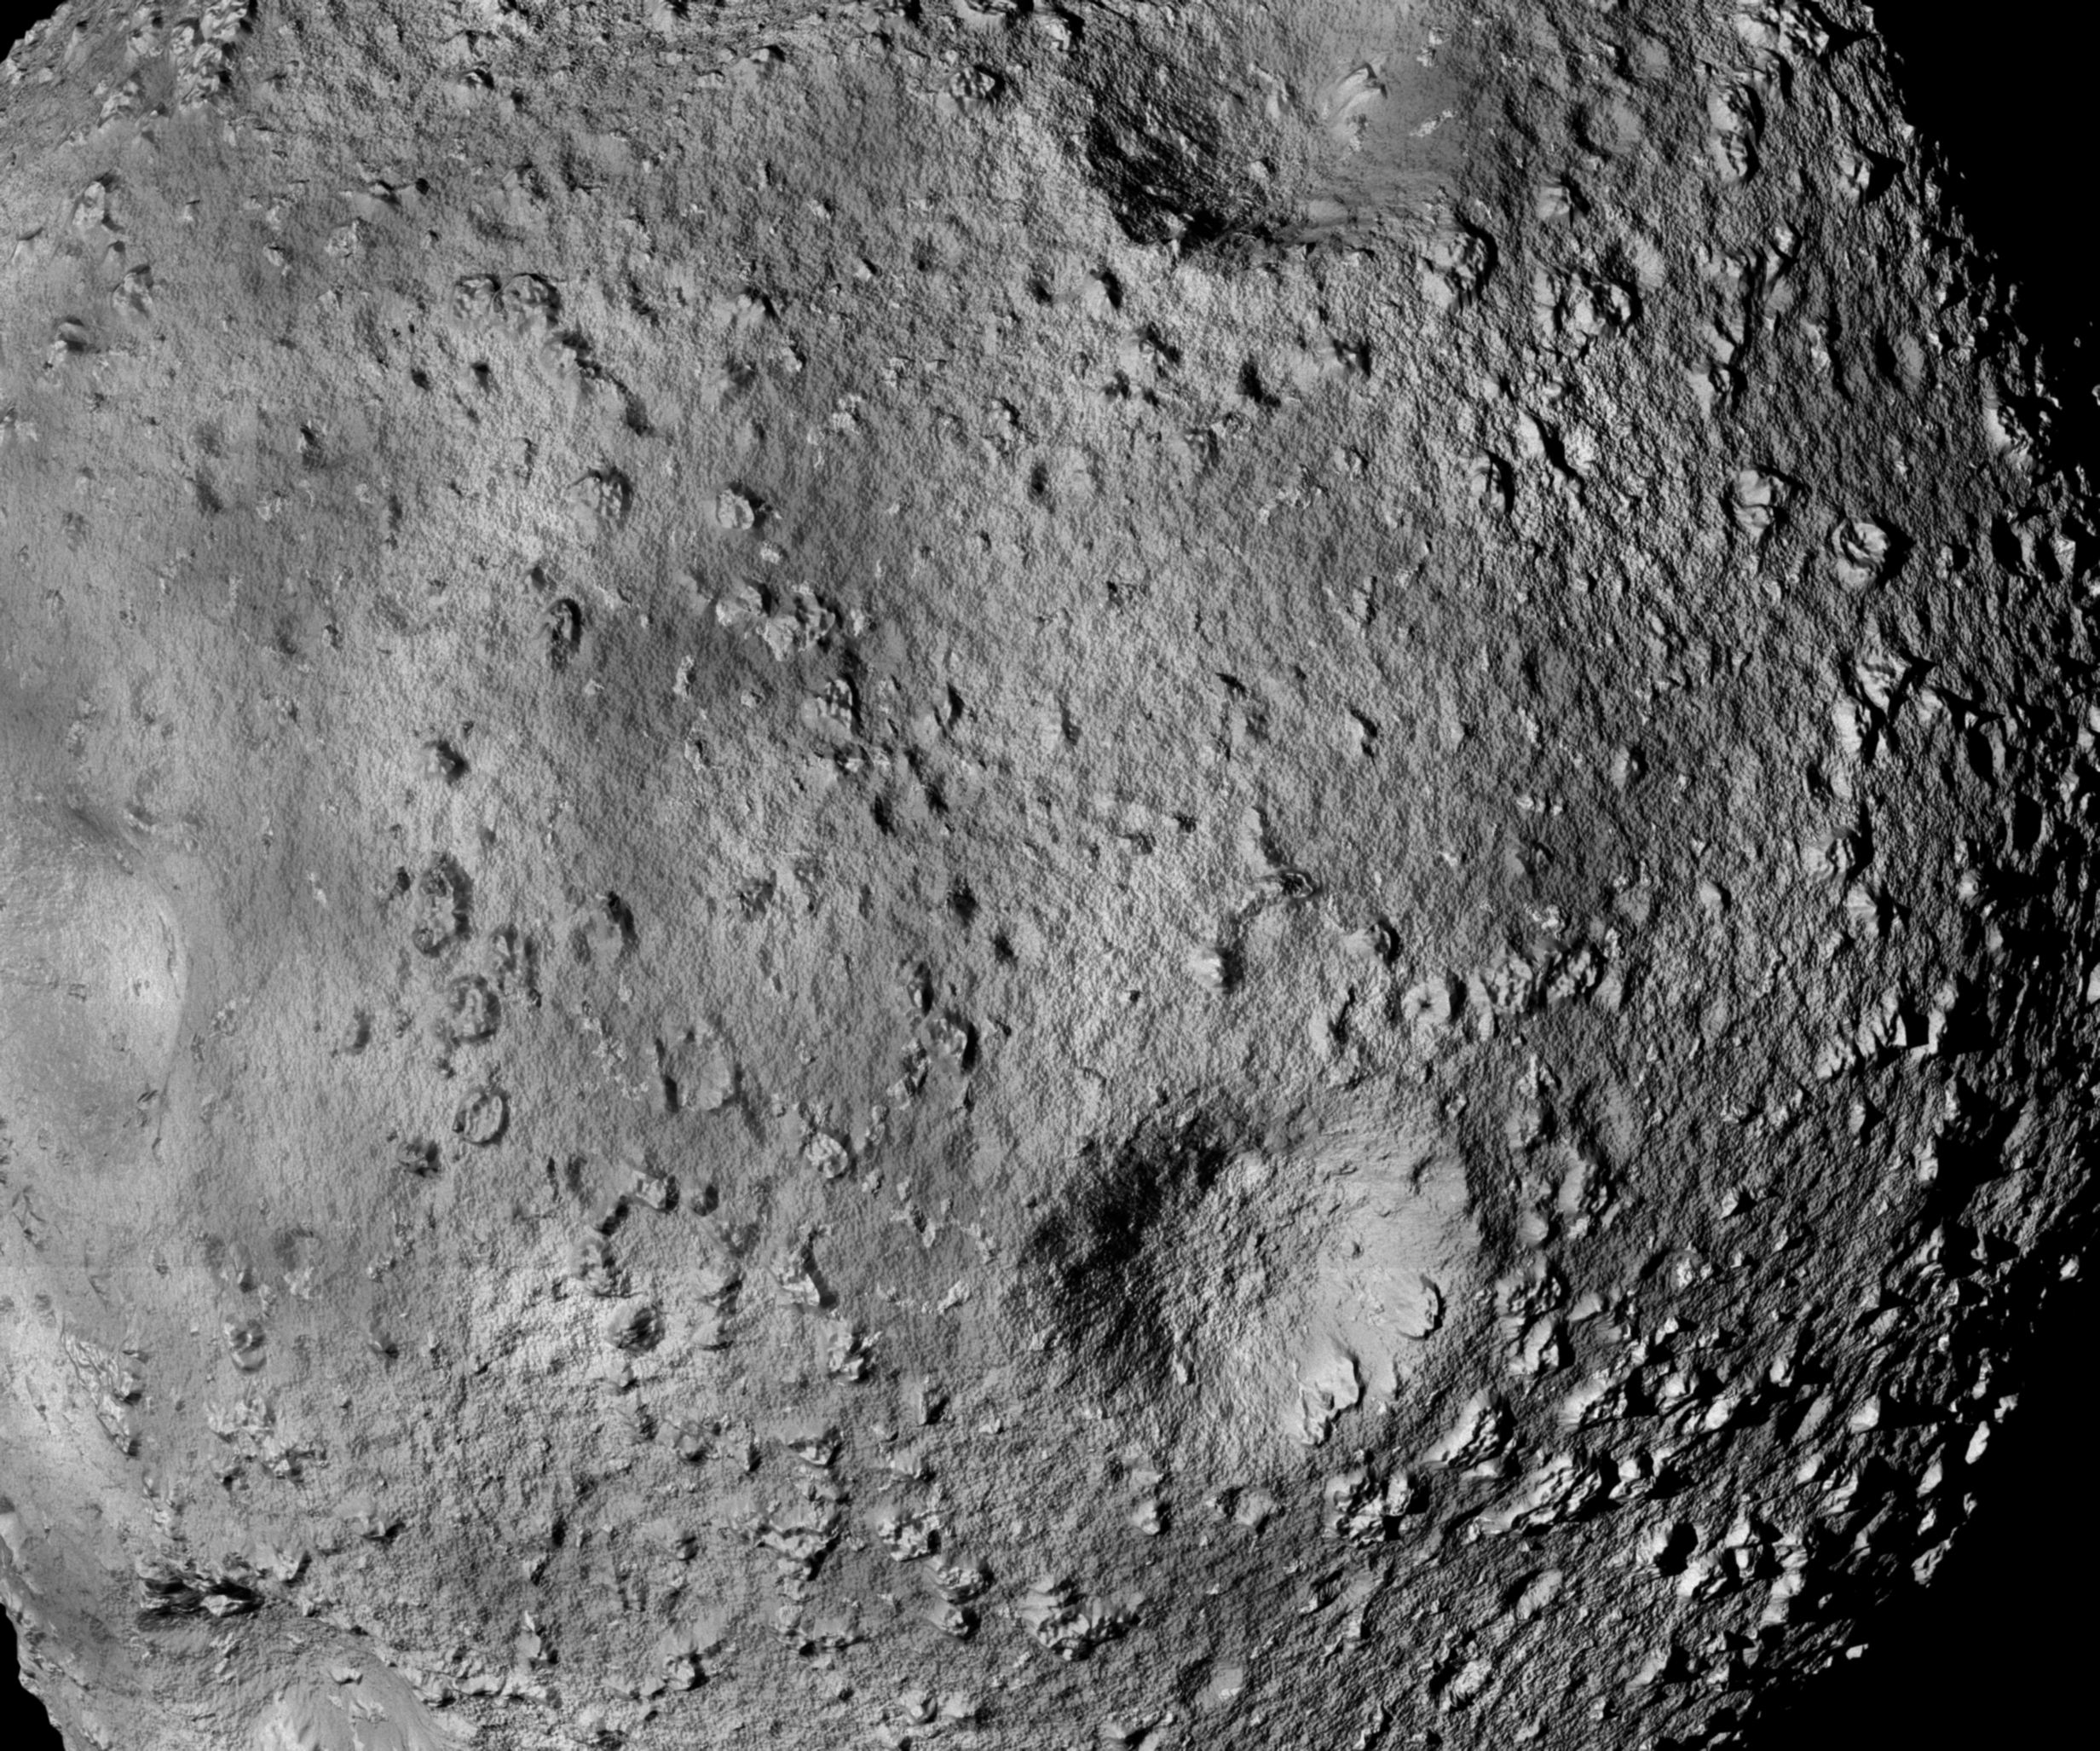
\includegraphics[width=\textwidth]{doc/thesis/0_figures/procedural_terrain/orig.png}
        \caption{}
        \label{fig:render_out_orig}
    \end{subfigure}
    \begin{subfigure}[b]{0.47\textwidth}
        \centering
        \includegraphics[width=\textwidth]{doc/thesis/0_figures/procedural_terrain/changed2.png}
        \caption{}
        \label{fig:render_out_changed}
    \end{subfigure}
    \\
    \begin{subfigure}[b]{0.47\textwidth}
        \centering
        \includegraphics[width=\textwidth]{doc/thesis/0_figures/procedural_terrain/main_moon.png}
        \caption{}
        \label{fig:render_out_main_moon}
    \end{subfigure}
    \begin{subfigure}[b]{0.47\textwidth}
        \centering
        \includegraphics[width=\textwidth]{doc/thesis/0_figures/procedural_terrain/bilobe2.png}
        \caption{}
        \label{fig:render_out_bilobe}
    \end{subfigure}
    \caption{Four rendered images using the Blender material used in \gls{sispo}. (a)~Render output with default shader parameters using the \gls{3d} model presented in Figure~\ref{fig:smooth_model}. (b)~Rendered image with changed shader parameters using the same model as in~(a). (c)~Render of a binary system with the same main body as in~(a) and default shader parameters. (d)~Bilobate body using default shader parameters.}
    \label{fig:render_out}
\end{figure}

Blender is interfaced using its Python bindings which need to be compiled manually (cf. Appendix~\ref{sec:app_setup} for setup instructions). A set of predefined settings is used for each scene while some parameters can be provided as input. The paths to the ".blend" files of models for the Sun, light reference and \gls{sssb} need to be provided in combination with the object name within the respective file.

Since images are composed and calibrated in a later step, described in Section~\ref{sec:composition}, the settings shown in Table~\ref{tab:color_space} are selected to not alter images with Blender while saving the raw rendered images.
\begin{table}[htb]
    \centering
    \caption{Blender settings that define the colour space and are fixed to not alter images after rendering.}
    \label{tab:color_space}
    \begin{tabular}{p{0.25\textwidth}|p{0.08\textwidth}|p{0.57\textwidth}}
        \textbf{Name}        & \textbf{Value} & \textbf{Description} \\ \hline
        Color mode           & RGBA           & Use RGB and alpha channel. \\
        Exposure             & 0              & Exposure in stops, applied before display transform. \\
        Sequencer colorspace & Raw            & Color space sequencer uses linear color space. \\
        View transform       & Raw            & No color space conversion. \\
        Look                 & None           & No artistic effect is applied before color space conversion. \\
        Film transparent     & True           & World background is transparent, i.e. alpha values can be used for image composition and proper occultation.
    \end{tabular}
\end{table}

The rendering performance of Blender can be configured depending on the available hardware and required image quality with the parameters presented in Table~\ref{tab:blender_settings_input}.
\begin{table}[htb]
    \centering
    \caption{Input parameters that that affect rendering performance and image quality in~\gls{sispo}.}
    \label{tab:blender_settings_input}
    \resizebox{\textwidth}{!}{%
        \begin{tabular}{p{0.15\textwidth}|p{0.15\textwidth}|p{0.7\textwidth}}
            \textbf{Parameter} & \textbf{Default Value} & \textbf{Description} \\ \hline
            device & AUTO & Device used for rendering, either "AUTO", \gls{cpu} or \gls{gpu}. "AUTO" attempts to use \gls{gpu}, if no \gls{gpu} is available uses \gls{gpu}. \\
            tile\_size & 512 (GPU)/ 128 (CPU)  & Size of a rendering tile. When rendering with a \gls{gpu} a bigger tile size tends to have better performance. When rendering with a \gls{cpu}, a smaller tile size tends to have better performance.\footnote{\url{https://docs.blender.org/manual/en/latest/render/cycles/render\_settings/performance.html?highlight=tile\%20size}} \\
            samples & 48 & Number of samples rendered per pixel.\\
        \end{tabular}
    }
\end{table}

Due to problems during rendering, the Blender scenes are scaled to kilometres instead of metres. I.e. one Blender unit corresponds to \SI{1}{\kilo\meter}. This is the only deviation from SI base units within the software.

\subsubsection{Star Rendering} \label{sec:stars}
The background stars are rendered based on the star catalogue \gls{ucac4}. This catalogue includes stars up to magnitude 16. The \gls{fov} is determined based on the spacecraft camera in the \textit{SssbOnly} scene since this camera provides the \gls{fov} of the spacecraft instrument. The edges of the \gls{fov} are calculated using Equation \ref{eq:fov_edge}. 
In the next step, we retrieve the list of stars that are visible in the \gls{fov}. The interface for the \gls{ucac4} is a commandline tool u4test.exe~\cite{gray}. This interface however requires that the \gls{fov} is input as right ascension \gls{ra}, declination \gls{de}, width and height.
The conversion of the vectors into their respective right ascension and declination is a transform between Cartesian coordinates to spherical coordinates. Their relation is defined as
\begin{align}
    \delta = \arcsin{(z)}, \label{eq:declination} \\
    \alpha_r = \arccos{\left(\frac{x}{\cos{\delta}}\right)} + \pi, \label{eq:right_ascension}
\end{align}
where \gls{de} is the declination, \gls{ra} the right ascension, $x$ is the x-coordinate and $y$ is the y-coordinate. Using this information the star catalogue returns a list of visible stars with their right ascension and declination as well as their magnitude.

The star background is created by generating an image with four times the size of final image. The coordinates are converted from the right ascension and declination of each star into pixel coordinates of the image frame using Equation \ref{eq:pix_conversion}. The pixel coordinates are multiplied with two to fit the oversized image.

The pixel value of each colour channel is set to the flux calculated from the magnitude as defined in Equation \ref{eq:mag_flux}. The resulting image is Gaussian filtered and down-sampled to the final image size using local means (cf. Section~\ref{sec:t_downsample}). Star background images are stored in the OpenEXR format with all alpha channel values equal to one. An example image is presented in Figure~\ref{fig:star_rendering}.

\begin{figure}[htb]
    \centering
    \includegraphics[width=\textwidth]{doc/thesis/0_figures/star_rendering/Stars_2017-08-15T115856-171000.png}
    \caption{Rendered star map containing several thousands stars.}
    \label{fig:star_rendering}
\end{figure}

\subsubsection{Image Composition} \label{sec:composition}
Rendered images of Blender vary in absolute light intensity thus requiring calibration. Since the star maps are not rendered in Blender, the raw images need to be combined. Optionally, the combined images can be transformed to a specified bit depth of a \gls{ccd} (cf. instrument input parameters in Table~\ref{tab:inst_input}). Hence, the composition process has two steps and an optional third step. 

First, the \gls{sssb} image and the star background are calibrated. In the second step, these images are combined to create a \gls{sssb} image with star background where stars are occluded by the \gls{sssb} nucleus. For calibration, the Blender output is normalised by comparing the theoretical and rendered intensity of a calibration disk in the same conditions.

The starting point for composition is a set of four images with the prefixes \textit{SssbOnly}, \textit{SssbConstDist}, \textit{LightRef} and \textit{Stars}. An example set is shown in Figure~\ref{fig:comp_imageset}. \textit{SssbOnly} represents the view from the spacecraft instrument. \textit{SssbConstDist} is a follower camera at a constant distance of \SI{1000}{\kilo\meter} from the \gls{sssb}. \textit{LightRef} is a defined reference model. \textit{Stars} is an image of the star background. These images are then composed to a single final image.

\begin{figure}[htb]
    \centering
    \begin{subfigure}[b]{0.47\textwidth}
        \centering
        \includegraphics[width=\textwidth]{doc/thesis/0_figures/composition/SssbOnly_2017-08-15T115855-684000.png}
        \caption{}
        \label{fig:comp_sssbonly}
    \end{subfigure}
    \begin{subfigure}[b]{0.47\textwidth}
        \centering
        \includegraphics[width=\textwidth]{doc/thesis/0_figures/composition/SssbConstDist_2017-08-15T115855-684000.png}
        \caption{}
        \label{fig:comp_sssbconstdist}
    \end{subfigure}
    \\
    \begin{subfigure}[b]{0.47\textwidth}
        \centering
        \includegraphics[width=\textwidth]{doc/thesis/0_figures/composition/LightRef_2017-08-15T115855-684000.png}
        \caption{}
        \label{fig:comp_lightref}
    \end{subfigure}
    \begin{subfigure}[b]{0.47\textwidth}
        \centering
        \includegraphics[width=\textwidth]{doc/thesis/0_figures/composition/Stars_2017-08-15T115855-684000.png}
        \caption{}
        \label{fig:comp_stars}
    \end{subfigure}
    \caption{Example set of images used for composition to the final rendering output. (a)~\textit{SssbOnly} image which represents the instrument \gls{fov}. (b)~\textit{SssbConstDist} image of a camera that follows the nucleus at a constant distance. (c)~\textit{LightRef} scene which contains the light reference used for calibration. (d)~\textit{Stars} image which represents the star background in the instrument \gls{fov}.}
    \label{fig:comp_imageset}
\end{figure}

Photometric calibration is based on the V-band of the \gls{ubv} as described in Section~\ref{sec:photo_cal}. While the \gls{ubv} was created before \glspl{ccd} were commonly used in imaging and therefore does not account for the higher sensitivity in the red and infrared spectrum of \glspl{ccd}, it was selected because it is easy to implement.

The calibration reference is the solar photon flux in the V-band. The Sun has a magnitude $m_{\astrosun} = -26.74$ at a distance of \SI{1}{\astronomicalunit}. Using Equation~\ref{eq:comp_flux_0mag} and the constants for the V-band from Table~\ref{tab:ubv_constants}, the solar photon flux density at \SI{1}{\astronomicalunit} becomes $F_{0,\astrosun} = \SI{4.36715206e+20}{\per\second\per\square\meter}$.
 
Since the spacecraft is normally not at exactly \SI{1}{\astronomicalunit}, this flux density is scaled using an inverse square law defined as
\begin{align}
    F_d = F \times \left(\frac{\SI{1}{\astronomicalunit}}{d}\right)^2, \label{eq:inverse_square}
\end{align}
where \gls{flux_scaled} is the scaled photon flux density, \gls{flux_d} is the flux density at \SI{1}{\astronomicalunit} and \gls{d} is the spacecraft's distance from the Sun in \SI{}{\astronomicalunit}.

In the next step, the reference photon flux for one pixel is calculated using Equation \ref{eq:comp_flux_pix} and the scaled photon flux density $F_d$.

To obtain the calibration factor for each pixel of the \gls{sssb} image, Equation \ref{eq:comp_cal_fac} is used. The reference intensity of the image is calculated as the mean intensity of $\SI{70}{}\times\SI{70}{}$ pixels of the centre of the light reference image.

In case the rendered image is far away from the \gls{sssb} nucleus, the visible size of the \gls{sssb} on the image is too small to be used for calibration. In such a case, a point source \gls{sssb} image is generated and used for calibration along with the \textit{SssbConstDist} image. The point source is necessary if the \gls{sssb}'s nucleus is only a few pixels of the image, since then intensities are not rendered correctly. The point source image is created by Gaussian filtering a single white pixel at the centre of an oversized image. The image is oversized by a factor of five, and then down-sampled to the original size using local means as described in Section~\ref{sec:t_downsample}. In this case the l

For the star background, every pixel value \gls{v} is calibrated using
\begin{align}
        v = v_0 \times F_0 \times A \times \frac{F_{stars}}{S_{stars}}, \label{eq:comp_cal_starmap}
\end{align}
with \gls{v_0} being the original pixel value, \gls{flux_0} being the flux at a magnitude \gls{m}$ = 0$, \gls{aperture} being the aperture area, \gls{flux_stars} being the total flux of visible stars, and \gls{s_stars} being the summed pixel value of one channel of a star map.

The star background and the calibrated \gls{sssb} image are merged taking the alpha channels into account. Using the alpha channel information provides proper occultation of the star background by the nucleus. For this, the film\_transparent option of Blender is activated which makes the scene background transparent, i.e. alpha values are zero.

The composed image is then multiplied by the efficiency of the instrument. This efficiency includes all efficiencies to convert incoming photon flux into pixel value, not only the \gls{ccd} quantum efficiency. Additionally, a diffraction pattern is added as well as noise which is based on a Poisson distribution. The diffraction pattern can be approximated with a Gaussian filter. The standard deviation for the Gaussian approximation of a diffraction pattern was found to be \gls{sigma} $\approx 0.45 \times$ \gls{lambda} $\times \frac{\gls{f}}{\gls{D}}$ when the Gaussian profile should contain the same energy as the diffraction pattern~\cite{Zhang2007GaussianModels}. Using this result, the standard deviation \gls{sigma} for Gaussian filtering is defined as
\begin{align}
    \sigma = 0.45 \times \lambda \times \frac{f}{D} \times \frac{m_d}{l_{pix}}, \label{eq:comp_sigma}
\end{align}
where \gls{lambda} is the observed wavelength, \gls{f} is the focal length, \gls{D} is the aperture diameter, \gls{l_pixel} is the length of one side of a pixel and \gls{m_d} is a multiplier for systems that are not diffraction limited (in our case \gls{m_d}~$= 2$, a perfectly diffraction limited system would have \gls{m_d}~$= 1$). The noisy image is scaled to an interval $[0,1]$ by dividing through the maximum value. In case a point source \gls{sssb} is used, the maximum value is clipped to five times the maximum of the reference if the maximum value of the merged image is above this threshold. The composed image using the data set shown in Figure~\ref{fig:comp_imageset} is presented Figure~\ref{fig:comp_composed}.

\begin{figure}[htb]
    \centering
    \includegraphics[width=\textwidth]{doc/thesis/0_figures/composition/Comp_2017-08-15T115854-575000.png}
    \caption{Composed image of the four images shown in Figure~\ref{fig:comp_imageset}. No stars are visible in the background because the nucleus is much brighter than the brightest background star.}
    \label{fig:comp_composed}
\end{figure}

In the additional third step, the image values are scaled to the bit depth of the \gls{ccd}. The current maximum permissible bit depth is \SI{16}{bit} due to an increase in code complexity for higher bit depths. This feature can be turned off by setting the with\_clipping parameter to false. This feature is used by default, since the aim is to realistically simulate the imaging capabilities of a spacecraft.

An additional feature is to add an information box in the lower right corner of the image including the distance to the \gls{sssb} and the date. This feature can be turned off by setting the with\_infobox parameter to false.

Throughout the composition process, the astropy package~\cite{robitaille2013astropy, price2018astropy} handles unit conversion between quantities. In addition, OpenCV~\cite{opencv_library} is used for down-sampling and Gaussian filtering during the composition process.

\subsection{Compression Package}
The compression module provides compression and decompression algorithms. These can be tested against different mission scenarios and image series to investigate the impact of compression and decompression on the scientific quality of the images. Table~\ref{tab:compression_format} shows the available compression and decompression algorithms.

\begin{table}[htb]
    \centering
    \caption{Lossless and lossy compression algorithms and image formats provided in \gls{sispo}. The implementation uses either native Python libraries$^{\ast}$~\cite{FoundationDataArchiving}, OpenCV$^{\dagger}$~\cite{opencv_library} or native OpenEXR$^{\ddagger}$~\cite{openexr}. The \gls{tiff} format can use either a lossless or lossy compression algorithm.}
    \label{tab:compression_format}
    \begin{tabular}{l|l}
        \textbf{Lossless Formats}  & \textbf{Lossy Formats} \\ \hline
        \gls{png}$^{\dagger}$      & \gls{jpeg}$^{\dagger}$  \\
        OpenEXR$^{\ddagger}$       & \gls{jp2}$^{\dagger}$   \\
        bzip2$^{\ast}$             & \gls{tiff}$^{\dagger}$  \\
        gzip$^{\ast}$              &                \\
        \gls{lzma}$^{\ast}$        &                \\
        zlib$^{\ast}$              &     \\
        \gls{tiff}$^{\dagger}$     &  
    \end{tabular}
\end{table}

Independent of the algorithm, files are handled equally. The images are loaded into NumPy arrays inside Python to have a common raw format. Before encoding, the information is reduced to \SI{8}{\bit} since the reconstruction module only reads images with \SI{8}{\bit} colour depth correctly. Images are encoded with the respective algorithm and converted into a binary stream. A copy of this data is saved as a file in the raw folder. The raw binary data is then converted back to a NumPy array and decoded to retrieve as much information as possible. Finally, the compressed and decompressed data is stored as a \gls{png} file to not lose any further information.

The formats \gls{png}, \gls{jpeg}, \gls{jp2} and tiff are implemented using OpenCV. There are various settings for each format\footnote{A detailed description can be found at \url{https://docs.opencv.org/4.1.2/d4/da8/group__imgcodecs.html\#ga292d81be8d76901bff7988d18d2b42ac}}.

The most important input parameter that is relevant to all algorithms is the "level" argument in "settings" which describes either the compression level (from 1 to 9 for bz2, gzip, \gls{lzma}, zlib and \gls{png}, higher meaning more compression) or the quality level (from 1 to 10 for \gls{jpeg} and 0.01 to 10 for \gls{jp2}, higher meaning better quality and less compression). Other input parameters to the compression package are presented in Table~\ref{tab:compression_settings}.

\begin{table}[htb]
    \centering
    \caption{Input parameters that define the compression behaviour in~\gls{sispo}.}
    \label{tab:compression_settings}
    \begin{tabular}{p{0.1\textwidth}|p{0.14\textwidth}|p{0.65\textwidth}}
        \textbf{Name} & \textbf{Default Value} & \textbf{Description} \\ \hline
        algo    & \gls{png}          & Compression algorithm, for a list of available algorithms see Table~\ref{tab:compression_format}\\
        settings    & \{"level": 9\} & Python dictionary including all settings for compression algorithms. For a description of the possible settings see the code or documentation of the providing library. \\
        img\_ext    & \gls{png}          & Image extension to search for when loading images for compression. 
    \end{tabular}
\end{table}

The compression and decompression has a simple implementation of multi-threading to run several image compression and decompression runs concurrently to reduce execution time. Images are only loaded during the compression and decompression process and are removed from memory directly afterwards.

\subsection{Reconstruction Package}
The reconstruction module can be used to generate a \gls{3d} model of an object using a series of images. It provides a full Multi-View Stereo reconstruction data process pipeline. To achieve this, two libraries are used and combined and called using python. The first library is \gls{omvg}~\cite{openMVG}. The second library is \gls{omvs}~\cite{openMVS}. 
The common steps for the complete pipeline is comprised of the following steps:
\begin{enumerate}
    \item Read in images [ImageListing in \gls{omvg}]
    \item Compute visual features [ComputeFeatures in \gls{omvg}]
    \item Match computed features between different images [MatchFeatures in \gls{omvg}]
    \item Generate point cloud from matched features [IncrementalSfM in \gls{omvg}]
    \item Export to \gls{omvs} format [openMVG2openMVS in \gls{omvg}]
    \item Increase number of points in point cloud [DensifyPointCloud in \gls{omvs}]
    \item Create a mesh from the point cloud [ReconstructMesh in \gls{omvs}]
    \item Refine the generated mesh [RefineMesh in \gls{omvs}]
    \item Apply texture to mesh to create final \gls{3d} model [TextureMesh in \gls{omvs}]
\end{enumerate}

\gls{omvg} and \gls{omvs} can be controlled with numerous parameters. All parameters have default values in \gls{sispo} itself which sometimes differ from the default settings of the software packages. These were adapted since they provide better results in the relevant scenarios.

During the image listing step, the spacecraft positions from the simulations are added as motion priors for improving the stability of the \gls{sfm} algorithms.

The reconstruction is based on two incremental and one global \gls{sfm} approach that \gls{omvg} provides. All three algorithms are executed and the number of reconstructed points are compared. The result containing the most points is exported to the \gls{omvs} format for further processing. None of the residuals are taken into account which is why this selection method might choose the highest quality point cloud due to a possible high number of outliers. Hence, if the result of the reconstruction is considered bad, it can be attempted to use one of the other results.

The algorithm used for reconstruction by IncrementalSfM2 is non-deterministic, i.e. results differ between runs on the same data sets. Hence, IncrementalSfM2 should be executed several times and the best result should be selected~\cite{Pajusalu2019CharacterizationMapping}.

\Gls{sispo} saves intermediate results which show steps of the reconstruction process, starting from the sparse point cloud and ending in the textured \gls{3d} model. Figure~\ref{fig:recon_steps} shows example images of the intermediate results. It shows how first sparse results are created which are then post-processed to increase the level of detail.

\begin{figure}[htbp]
    \centering
    \begin{subfigure}[b]{0.4\textwidth}
        \centering
        \includegraphics[width=\textwidth,height=5.95cm]{doc/thesis/0_figures/models_quality/100_1/120_100_1_points2.png}
        \caption{}
        \label{fig:recon_step_point}
    \end{subfigure}
    \begin{subfigure}[b]{0.4\textwidth}
        \centering
        \includegraphics[width=\textwidth,height=5.95cm]{doc/thesis/0_figures/models_quality/100_1/120_100_1_dense1.png}
        \caption{}
        \label{fig:recon_step_dense}
    \end{subfigure}
    \\
    \begin{subfigure}[b]{0.4\textwidth}
        \centering
        \includegraphics[width=\textwidth,height=5.95cm]{doc/thesis/0_figures/models_quality/100_1/120_100_1_mesh1.png}
        \caption{}
        \label{fig:recon_step_mesh}
    \end{subfigure}
    \begin{subfigure}[b]{0.4\textwidth}
        \centering
        \includegraphics[width=\textwidth,height=5.95cm]{doc/thesis/0_figures/models_quality/100_1/120_100_1_refine2.png}
        \caption{}
        \label{fig:recon_step_refine}
    \end{subfigure}
    \\
    \begin{subfigure}[b]{0.4\textwidth}
        \centering
        \includegraphics[width=\textwidth,height=5.95cm]{doc/thesis/0_figures/models_quality/100_1/120_100_1_texture1.png}
        \caption{}
        \label{fig:recon_step_texture}
    \end{subfigure}
    \begin{subfigure}[b]{0.4\textwidth}
        \centering
        \includegraphics[width=\textwidth,height=5.95cm]{doc/thesis/0_figures/models_quality/100_1/120_100_1_img1.png}
        \caption{}
        \label{fig:recon_step_img}
    \end{subfigure}
    \caption{Example images of intermediate results of the reconstruction pipeline. (a)~Sparse point cloud created by \gls{omvs}. (b)~Point cloud densified with \gls{omvs}. (c)~Mesh created from the dense point cloud in~(b) using \gls{omvs}. (d)~Refined mesh based on the mesh created in~(c) using \gls{omvs}. (e)~Mesh textured using \gls{omvs}. (f)~Reference image for comparison with the textured mesh.}
    \label{fig:recon_steps}
\end{figure}

The most important goal for the reconstruction pipeline is to reconstruct a model. However, \gls{sispo} attempts to create the most detailed model possible by densifying the point cloud and refining the mesh. In case one of these two processes is not run successful, \gls{sispo} continues with either the sparse point cloud or the sparse mesh.

\subsection{User Interface}
\Gls{sispo} can be imported as a Python package and therefore the user interface is a Python console. The settings for the three sub-packages along with general settings of \gls{sispo} are stored in a \gls{json} file. After importing, \gls{sispo} can be started by one of two equivalent functions, either sispo.run() or sispo.main(). An example of a definition.json file is given in the repository in the data/input folder. While this example provides the most important settings, there are more settings that can be used. Especially the software packages used for \gls{sfm} have many default settings which can be customised. For an explanation of all parameters, refer to the documentation of the respective software or Python package.

The high-level behaviour of \gls{sispo} can be controlled using a set of flags presented in Table~\ref{tab:cli_args}.
\begin{table}[htb]
    \centering
    \caption{Input flags to control high-level behaviour of \gls{sispo}.}
    \label{tab:cli_args}
    \resizebox{\textwidth}{!}{%
        \begin{tabular}{p{0.24\textwidth}|p{0.32\textwidth}|p{0.16\textwidth}|p{0.27\textwidth}}
            \textbf{Name} & \textbf{Variable Name} & \textbf{Default Value} & \textbf{Description} \\ \hline
            --help & & --- & Prints list of arguments with hints \\
            -i & i & definition.json & Path to a definition file that defines the settings \\
            -v & v & False & Flag to use verbose output, i.e. logging information will also be displayed to console \\
            --profile & profile & False & Flag to use Python's cProfile to profile \gls{sispo} execution \\
            --no-sim & with\_sim & True & Flag to skip simulation step\\
            --no-render & with\_render & True & Flag to skip rendering step\\
            --no-compression & with\_compression & True & Flag to skip compression \\
            --no-reconstruction & with\_reconstruction & True & Flag to skip reconstruction \\
            --sim-only & sim\_only & False & Flag to do simulation step \\
            --sim-render-only & sim\_render\_only & False & Flag to do simulation and rendering steps \\
            --render-only & render\_only & False & Flag to do rendering step\\
            --compress-only & compress\_only & False & Flag to do compression step \\
            --reconstruct-only & reconstruct\_only & False & Flag to do reconstruction step \\
            --compress-reconstruct-only & compress\_reconstruct\_only & False & Flag to do compression and reconstruction steps
        \end{tabular}
    }
\end{table}

\Gls{sispo} can be installed as a Python package via pip. This method provides a \gls{cli} which accepts the arguments presented in Table~\ref{tab:cli_args}.

\subsection{Performance}
the performance of \gls{sispo} and its components was analysed during the development to find code section that substantially increase execution time. While reducing the number of dependencies, it was ensured that the performance does not degrade.

\subsubsection{Overall Performance}
\gls{sispo} was executed on a machine running Linux Ubuntu~18.04.03~LTS, \SI{16}{\giga\byte} of \gls{ram}, Intel\textsuperscript{\textregistered}~Core\texttrademark~i7-8700 processor with \SI{6}{} cores and an NVIDIA\textsuperscript{\textregistered}~GeForce~GTX~1080 with \SI{8}{\giga\byte} memory.

Two test cases were analysed with the parameters and main results given in Table~\ref{tab:profiles}. The performance assessment of these complete \gls{sispo} runs shows that the most time consuming part is rendering. More than \SI{90}{\percent} of the overall execution time is dedicated to rendering. With only \SI{5}{\percent} to \SI{6}{\percent} used for rendering and less than \SI{1}{\percent} for compression, these steps do not account for much of the overall execution time. Moreover, the total execution time shows differences for the two test cases because of the different apparent size of the \gls{sssb}. Based on the two examples, the execution time for reconstruction is affected even stronger than rendering by decreasing fly-by distance.
Since most of the time of a simulation is spent rendering, improving the performance of \gls{sispo} further requires improving the performance of the rendering process either by changing the parameters or improving the shader implementation.

\begin{table}[htb]
    \centering
    \caption{Summary of two profiles obtained while executing a complete run of \gls{sispo}, i.e. rendering, compression and reconstruction. More than \SI{90}{\percent} of total time is spent rendering images.}
    \label{tab:profiles}
    \resizebox{\textwidth}{!}{%
        \begin{tabular}{l|l|l|l|l|l|l|l|l}
            \textbf{Distance} & \textbf{\gls{sssb} size} & \textbf{Total time} & \multicolumn{2}{l}{\textbf{Rendering}} & \multicolumn{2}{|l}{\textbf{Compression}} & \multicolumn{2}{|l}{\textbf{Reconstruction}} \\
            \textbf{[\SI{}{\kilo\meter}]} & \textbf{[\SI{}{\kilo\meter}]} & \textbf{[\SI{}{\second}]} & \textbf{[\SI{}{\second}]} & \textbf{[\SI{}{\percent}]} & \textbf{[\SI{}{\second}]} & \textbf{[\SI{}{\percent}]} & \textbf{[\SI{}{\second}]}  & \textbf{[\SI{}{\percent}]} \\ \hline
            200 & 10 & 346939.8 & 325834.6 & 93.9 & 55.6 & 0.2 & 21048.2 & 6 \\
            400 & 10 & 212209.4 & 201443.2 & 94.9 & 24.7 & 0.1 & 10740.1 & 5.1
        \end{tabular}%
    }
\end{table}

\subsubsection{Image Processing Benchmark} \label{sec:cvskimage}
The original source code used the \gls{skimage} and OpenCV libraries concurrently. In order to reduce the number of dependencies, the relevant functions of the two libraries were compared. The parameters for the OpenCV functions were selected to create the same behaviour as the respective \gls{skimage} function. The benchmark compares the performance of the Gaussian filter and image resizing using local means as described in Section~\ref{sec:t_downsample}. Five images are selected for the benchmark. The image set is presented in Appendix~\ref{sec:app_cvskimage}. Two star maps were selected due to the large variance in the number of visible stars. The selected images contain 1804 (Stars1) and 51338 stars (Stars2).

Two computers are used for the benchmark. A laptop with \SI{8}{\giga\byte} \gls{ram}, an Intel\textsuperscript{\textregistered}~Core\texttrademark~i7-6700HQ with \SI{4}{} cores at \SI{2.6}{\giga\hertz} and Windows 10. The second is a workstation computer with \SI{16}{\giga\byte} of \gls{ram}, an Intel\textsuperscript{\textregistered}~Core\texttrademark~i7-8700 processor with \SI{6}{} cores at \SI{3.2}{\giga\hertz} and Ubuntu~18.04.3~LTS.

To compare the performance between the two libraries the ratio of execution time is used. The ratio is defined as
\begin{align}
    Ratio = \frac{T_{skimage}}{T_{opencv}}, \label{eq:bm_exec_ratio}
\end{align}
where \gls{T}$_{skimage}$ is the execution time of \gls{skimage} and \gls{T}$_{opencv}$ is the execution time of OpenCV. Each command is executed and timed for 1000 times. The lowest value is chosen as the result, since higher values are rather influenced by other processes running on the respective machine than the relevant code snippet itself~\cite{timeit2020}.

Figure~\ref{fig:bm_comparison} shows execution time ratios and averages for the image set. A ratio larger than one represents a longer execution time of \gls{skimage}. On average, OpenCV outperforms \gls{skimage} for both tests on both computers. The maximum absolute difference between pixel values of images is \SI{1.486e-6}{} and \SI{7.153e-7}{} for the Gaussian filtered and the resized images respectively. Such differences are not relevant for image colour depths of up to \SI{16}{bit}.

%Maximum error gauss:  1.4864218655930017e-06
%Maximum error resize:  7.152557373046875e-07

\begin{figure}[htb]
    \centering
    \begin{subfigure}[b]{0.47\textwidth}
        \centering
        \includegraphics[width=\textwidth]{doc/thesis/0_figures/cv_skimage/Comparison_Gaussian}
        \caption{}
        \label{fig:bm_comparison_gauss}
    \end{subfigure}
    \begin{subfigure}[b]{0.47\textwidth}
        \centering
        \includegraphics[width=\textwidth]{doc/thesis/0_figures/cv_skimage/Comparison_Resize}
        \caption{}
        \label{fig:bm_comparison_res}
    \end{subfigure}
    \caption{Comparison of execution time ratios of (a) Gaussian filtering and (b) resizing five images using OpenCV and \gls{skimage} on two computers. Values $> 1$ correspond to OpenCV being faster. The mean values are given in the legend.}
    \label{fig:bm_comparison}
\end{figure}

OpenCV has a performance advantage over the \gls{skimage} library, hence only OpenCV is being used. OpenCV might also be used to replace the OpenEXR dependency in the future, if the OpenEXR implementation of OpenCV includes alpha channel support\footnote{A GitHub issue was created at \url{https://github.com/YgabrielsY/sispo/issues/128} that links to the relevant OpenCV GitHub issue.}.